% main.tex
%
% This file groups together all of the chapters, which are stored as neighboring files in this
% directory. It also establishes the general formatting of the paper, as specified here:
%   https://www.cs.ox.ac.uk/teaching/courses/projects/handbook/Project%20Handbook%202021.pdf
% And finally, it defines a number of commands that are used elsewhere.

\documentclass[12pt]{article}
\usepackage[paper=a4paper,margin=3cm]{geometry}
\frenchspacing

\usepackage[utf8]{inputenc}
\usepackage{amsmath}
\usepackage{bm}
\usepackage{changepage}
\usepackage{float}
\usepackage{graphicx}
\usepackage{hyperref}
\usepackage{natbib}
\usepackage{pgfplots}
\usepackage{textcomp}
\usepackage{tikz}
\usepackage{xcolor}

% A selection of colors making up a pastel-like palette, just so everything's a bit more pleasing on
% the eye.
\definecolor{softgrey}{HTML}{808080}
\definecolor{softblue}{HTML}{4C70D4}
\definecolor{softgreen}{HTML}{26AB56}
\definecolor{softyellow}{HTML}{D9D44C}
\definecolor{softorange}{HTML}{D67331}
\definecolor{softred}{HTML}{CF463C}

% Used as an "almost" `softblue`
\definecolor{softsoftblue}{HTML}{698DF0}

% Usage: \code{ <text> }
%
% Produces inline code formatting.
\newcommand{\code}[1]{\texttt{#1}}

% Usage: \breakpars
%
% Adds a little bit of space in between paragraphs.
\newcommand{\breakpars}{\vspace{0.1in}}

% Usage \norm { math mode content }
%
% Outputs the norm / magnitude / absolute value of the contents - || contents ||
% Taken from https://tex.stackexchange.com/a/107190
\newcommand{\norm}[1]{\left\lVert#1\right\rVert}

% Usage \tightbox { content, e.g. \includegraphics{..} }
%
% Creates a box that exactly borders the content
\newcommand{\tightbox}[1]{%
    {\setlength{\fboxsep}{0pt}\fbox{#1}}%
}

\newcommand{\todo}[1]{%
    \begin{adjustwidth}{-0.5cm}{-0.5cm}{%
        \noindent\textcolor{red}{Todo:} \bf{#1}%
    }\end{adjustwidth}%
}

\begin{document}

% Title page

\begin{titlepage}
\begin{center}
    \Huge
    \textbf{Title}

    \vspace*{0.4cm}
    \LARGE
    Subtitle

    \vspace{1.5cm}
    \textbf{Max Sharnoff}

    Trinity 2022 \\
    candidate number \\
    BA Computer Science

\end{center}
\end{titlepage}

% Blank page
\newpage\ \addtocounter{page}{-1} \thispagestyle{empty}

% Abstract
\newpage
% Abstract.tex
%
% vim: set ft=tex:

{\Large \textbf{Abstract}}

\vspace{0.5cm}

Detecting changes in human lung morphology and determining its effects on lung function requires
significant time committment per patient, so statistical analysis on many individuals is infeasible.
Computational models of the lung are therefore a natural choice for researching the effects of
altered lung morphology, with reference to existing lung function tests.

Accurate computational models also allow investigation into properties of the lungs that cannot
feasibly be measured; e.g., increased internal stress in one location from damaged airways
elsewhere.

This paper builds on recent advancements in modelling airflow in the lungs (\textlangle reference to
Foy\textrangle) to produce an efficient, accurate model of the lungs that supports simple
alterations to the simulated morphology.  We then use this model to determine the strains placed on
the rest of the lungs by various kinds of constricted or damaged airways.


% Table of contents
\newpage
\tableofcontents

\newpage
% Ch1-introduction.tex
%
% vim: set ft=tex:
\section{Introduction}

Outline (generally pretty short; most of the introductory information is in ``Background''):

\begin{itemize}
    \item Motivation -- the lungs are generally pretty complicated, and respiratory diseases are all
        too common. It would be really useful to get more insight into what happens as they move
        further away from ``normal'' functioning, but the ethics board wouldn't be happy if we
        started damaging patient's lungs ``for science''. So computational models are a natural
        solution. Historically, they've been difficult to 
    \item Contributions to the field -- basically, a new tool to play with. This should be really
        useful to people looking to find new results about \textit{how} the lungs get impacted by
        various diseases. To kick-start this, we've investigated the effects of a couple \textlangle
        diseases?  changes in lung morphology? \textrangle
\end{itemize}


\newpage
% Ch2-background.tex
%
% vim: set ft=tex:
\section{Background}

\subsection{Physiology of the lungs}

At a high level, the physiology of the lungs can be divided into the few most significant
structures. This section does not discuss pulmonary blood circulation, or the mechanics of gas
exchange~--~this paper is primarily concerned with the flow of air in and out of the lungs.

The flow of air into the lungs begins with the diaphragm, a muscle below the lungs that contracts to
increase the volume of the \textit{thoracic cavity} (where lungs are housed). This increase in
volume causes the negative pressure that drives inspiration. Correspondingly, typical expiration is
driven by relaxation of the diaphragm and the associated increase in pressure in the thoracic
cavity.

Air flows into the body through the nose and mouth, meeting the trachea at the larynx, in the neck.
The trachea splits into the left and right bronchi~--~connecting to the left and right lungs
respectively. The bronchi split into a binary tree of progressively smaller bronchial tubes (the
\textit{tracheobronchial tree}), with the \textit{generation} of a bronchial tube referring to the
number of branches between it and the larynx. The smallest bronchial tubes terminate in a small
number of acini, small clusters of alveoli. Alveoli are the small, spherical air sacs that act as
the sites of gas exchange with the blood. A core technique used in this paper is the approximation
of one or many acini as spherical air sacs themselves, further described in
\autoref{sec:approximating-lungs}. Typical dimensions for all of the structures above are given in
\autoref{tab:lung-sizes}.

% FIXME: ^ need sources here
% https://en.wikipedia.org/wiki/Lung#/media/File:Secondary-pulmonary-lobule-illustration.jpg
%  ^ good diagram
% https://pubmed.ncbi.nlm.nih.gov/472520/
%  ^ "A statistical description of the human tracheobronchial tree geometry"

Beyond the structure of the lungs, there are also a number of measures of volume. \textit{Tidal
volume} (TV) refers to the volume of air moved in or out of the lungs during a typical breath, and
\textit{functional residual capacity} (FRC) refers to the total volume of air remaining in the lungs
after a normal expiration.\footnotemark\ Typical values for TV and FRC are also given in
\autoref{tab:lung-sizes}.

% FIXME: ^ source = https://www.ncbi.nlm.nih.gov/books/NBK545177/
%   ^ useful: https://pubmed.ncbi.nlm.nih.gov/12773331/
%   ^         https://www.ncbi.nlm.nih.gov/pmc/articles/PMC5980468/

\footnotetext{
    \textbf{N.B.:} TV and FRC both describe typical breaths; there are analogous terms for maximum
    capabilities (\textit{vital capacity} (VC) and \textit{residual volume} (RV)). Also notable is
    \textit{total lung capacity} (TLC; equal to VC + RV). These are included here for context, but
    they are not necessary for understanding the experiments in this paper.
}

\begin{table}[h]
\centering
    \begin{tabular}{ |c|c|c| }
    \hline
        Metric & Mean value (adult female) & Mean value (adult male) \\
        \hline \hline
        Trachea length & todo & todo \\ % FIXME: fill in the chart lol
        Trachea radius & todo & todo \\
        Bronchus length & todo & todo \\
        Bronchus radius & todo & todo \\
        Acinus radius & todo & todo \\
        Alveolus radius & todo & todo \\
        \hline
        TV & todo & todo \\
        FRC & todo & todo \\
        \hline
\end{tabular}
\caption{
    Typical sizes of various lung structures and volumes. Larger structures and effects tend to be
    more different in proportion between average males and females.
}
\label{tab:lung-sizes}
\end{table}

\subsection{Clinical methods}

There are a number of relevant clinical methods for measuring lung function, many of which will be
discussed in this section. Despite the clinical utiltiy however, there are certain limitations to
these methods that make them less well-suited to research, namely: difficulty with establishing
causation and cost per datapoint (either monetary, temporal, or both).

Reservations aside, current clinical tools for measuring lung function can essentially be grouped
into three categories: exhalation measurement: spirometry and inert-gas washout; oscillometry: FOT
and IOS; or imaging techniques: CT, PET, and MRI.

\textit{Spirometry} measures the volume and flow from a patient's maximal exhalation (after maximal
inhilation), producing volume-flow and volume-time curves. It is simple to perform, but the reliance
on maximal exhalation gives it a particularly low sensitivity. \textit{Inert-gas washout} instead
floods the lungs with an inert gas (e.g.~\ce{SF_6} or \ce{^3He}) before continuously measuring the
concentration of the gas exhaled through normal breathing. Measurements are either made over many
breaths (\textit{multiple-breath washout} (MBW)) or just one (\textit{single-breath washout} (SBW)).
Both MBW and SBW have a number of indices typically produced from the data, which correlate with
many lung diseases.

Both \textit{forced oscillation technique} (FOT) and \textit{impulse oscillometry} (IOS) apply
oscillations at the mouth and measure the resulting airflow and pressure. FOT uses controlled
pulses whereas IOS uses pseudo-random noise. From this, estimates of resistance and inertance of the
lungs are made, which have correlations to diseases such as asthma and COPD.

Finally, we have the imaging techniques: \textit{Magnetic resonance imaging} (MRI), \textit{computed
tomography} (CT), and \textit{positron emission tomography} (PET). Beyond immediately-visible
ailments (e.g. foreign objects or fluid buildup), these methods can also be used to estimate the
ventilation of air in each voxel of the image~--~providing metrics that can quantify overall lung
function (and highlight specific regions where function is degraded). However, these methods are
typically expenive (MRI) or dangerous in large amounts (CT and PET) and the timeline of resolution
improvements means that high-resolution imaging has not been available for as long as other methods.
The costs associated with these methods and the relative recency of high-resolution versions has
meant that there is also a relative gap in the literature linking imaging results to respiratory
disease classification.

This final point is one of the key reasons why computational models are so useful; high costs or low
availability hinder new research, and computer simulation can provide a simpler, cheaper method for
testing ideas. It is difficult to obtain large amounts of data for analysis when the underlying
methods are expensive or time-consuming, relative to the amount of data produced.\footnotemark

\footnotetext{
    To be clear here: methods like spirometry are relatively cheap and not overly time-consuming,
    but the amount of data each test generates is small; establishing complex relationships may
    require large amounts of data, regardless of the type of test used.
}

Also of note is that all of the above techniques are strictly observation with respect to the
condition of the lungs. Analyzing the effects of various morphological changes within the lungs is
difficult without the ability to directly effect those changes, but forced changes to patient lung
morphology are typically both risky and unethical.

For those reasons, it is natural to turn to simulations -- in particular, computational models -- in
order to gain insight into impact on physiology and overall function from isolated changes within
the lungs.

\subsection{Prior computational models}

This section is unfortunately brief~--~historically, computational models have been limited by the
available resources (they still are) and data to base them on. From the beginning, simulating
``full'' fluid dynamics with the Navier-Stokes equations has been both unnecessary and out of reach;
reasonable assumptions can be made about the flow of air within the lungs to simplify modelling
(see: \autoref{sec:approximating-lungs}), and models have increased in complexity over time to match
advancements in the speed of computers.

Early models represented the lungs with just a few elastic chambers, but advancements in
physiological data (particularly from Weibel, 1963) allowed later models to generate larger models
of the lungs, with the size now singularly limited by computational capabilities.

More recently, models have been partially constructed with results from patient imaging (up to
generations 6-10) with later generations generated by the parameters from Webiel (1963).

\todo{ the ``Weibel, 1963'' above needs to actually be a reference }


\newpage
% Ch3-methods.tex
%
% vim: set ft=tex:
\section{Methods}

Broadly speaking, this section comes in two parts; first defining the more theoretical underpinnings
of the model used for simulation, followed by detail on the implementation in practice. There is
relatively little theory to discuss; much of it comes from prior work.\cite{Foy2018}

At a high level, we use a system of simultaneous equations to determine how the state of the
simulated lungs evolves, updating in discrete timesteps to give a close approximation to the way a
similar physical system would behave. \autoref{eq:volume-cons-naive} governs the
conservation of volume from one timestep to the next, which allows us to obtain greater numerial
stability than we might otherwise, e.g., with
$\text{volume}_{t+1} = \text{volume}_t + \text{flow} dt$.

Instead of a ``full'' fluid simulation (e.g., with the Navier-Stokes equations), we use a
one-dimensional simulation as shown in \citeauthor{Foy2018}, \citeyear{Foy2018}.

\subsection{Simultaneous Equations}

This section provides a summary and brief description of the four simultaneous equations that govern
the state of our system, the first of which is the following:

\begin{equation}
    P_{\text{parent}(i)} - P_i = R(i) Q_i
\end{equation}

\noindent
This specifies that the pressure differential between the distal end of branch $i$ and its parent
must equal the pressure from the resistance from the flow through this branch $i$. For the ``root''
branch, $P_{\text{parent}(i)}$ is the pressure at the trachea~--~typically atmospheric pressure.

The resistance term $R(i)$ is defined as following function, as given by Pedley et al. (1970):

\begin{equation*}
    R(i) = \frac{2 \mu L_i c}{\pi r_i^4} \left( \frac{4 \rho |Q_i|}{\mu \pi L_i} \right)^{\frac{1}{2}}
\end{equation*}

The parenthesized term corresponds to the Reynold's number of the flow, scaled by the ratio of the
diameter of the branch to its length $L_i$. $r_i$ is the radius of branch $i$, $\mu$ is the
viscosity of the air, and $c = 1.85$ is a correction constant.

The second equation ensures incompressibility; the flow through a bifurcation must equal the sum of
the flow through its children:

\begin{equation}
    Q_i = \sum Q_{\text{child}}
\end{equation}

\noindent
where each \textit{child} refers to any branch $c$ with $\text{parent}(c) = i$.

The third equation maintains that the volume of an acinar region changes with the flow into or out
of it for the given timestep:

\begin{equation}
    V_i^t = V_i^{t-1} + dt Q_i^t
\end{equation}

\noindent
where $dt$ is the timestep size, $t$ refers to the current timestep, and $V_i$ is the volume of the
acinar region of branch $i$.

The final equation defines the elastic force of each acinar region, relating the pressure it exerts
on its branch to the volume of the region itself and the pressure outside it:

\begin{equation} \label{eq:volume-cons-naive}
    P_i = \frac{1}{C_i} V_i + P_{pl}(t)
\end{equation}

\noindent
where $P_{pl}(t)$ is the pleural pressure (i.e. the ``pressure'' from the diaphragm, outside the
acinar region) at the current time and $C_i$ is the \textit{compliance} of the acinar region of
branch $i$. The pleural pressure changes over time to mimic human breathing patterns~--~hence why it
is parameterised by $t$.

\subsection{Modelling in the Abstract} \label{sec:modelling-in-the-abstract}

We use an \textit{implicit} Euler's method to model the system as it progresses: at each timestep,
our simulation updates its state to the value of an approximate solution to the system of equations
above. \autoref{eq:volume-cons-naive} provides the necessary bounds to make the method implicit,
giving us higher accuracy at the cost of implementation complexity.

To solve for an approximate solution at each timestep, we use Newton's method with $f_{\bm{S}}(\bm{x})$ as
defined below, iterating until $\norm{f_{\bm{S}}(\bm{x})}^2 \le tol$ and $\norm{dx}^2 \le tol$, with
a tolerance of $10^{-6}$. The two ``inputs''~--~$\bm{S}$ and $\bm{x}$~--~partition the state of the
model into the variables that are controlled externally (e.g.: pleural pressure, compliance) and
those that are calculated from the system state (e.g.: acinar volume, airflow). The definitions of
$\bm{x}$ and $f_{\bm{S}}$ are given by:

\begin{equation*}
    x = (P_i..., Q_i..., V_i...)
\end{equation*}

\begin{equation*}
    f_{\bm{S}}(\bm{x}) =
        \begin{bmatrix}
            P_{\text{parent}(i)} - P_i - R(i)Q_i \\
            \vdots \\
            Q_i - \sum Q_{\text{child}} \\
            \vdots \\
            V_i^t - V_i^{t-1} - dtQ_i^t \\
            \vdots \\
            P_i - P_{pl}(t) - \frac{1}{C_i} V_i \\
            \vdots \\
        \end{bmatrix}
\end{equation*}

Note that the values in $\bm{x}$ and equations in $f$ are repeated only as many times as fits; e.g.,
there are fewer acinar regions than total branches, so there are fewer components in $\bm{x}$ from
each $V_i$ than from each $Q_i$.

As $\bm{S}$ only exists in the abstract sense, we won't bother to define its structure; all that's
necessary to know is that it contains every variable referred to in $f$ that is not already given
explicitly by $\bm{x}$.

\breakpars

It's worth noting that in practice, the above definitions are only \textit{nearly} correct; a few
adjustments were made to the inputs and equations to mitigate limitations from floating-point
accuracy. These are discussed in the \hyperref[sec:units-and-numerical-stability]{next section}.

\subsection{Units \& Modified Equations for Numerical Stability} \label{sec:units-and-numerical-stability}

It is worth making explict the units used for each value in our simultaneous equations. After
careful consideration, these were considered to provide the best trade-off of familiar units and
those with values of magnitude close to one, where floating-point accuracy is maximized. As we will
see momentarily, the spread was still quite wide. The chosen units were:

{
    % Add a bit more spacing within the rows of the table
    \renewcommand{\arraystretch}{1.6}
    \begin{table}[h]
    \centering
    \begin{tabular}{ |c|c| }
        \hline
        Type of thing ??? & Units \\
        \hline \hline
        Distance & $\text{m}$ \\
        \hline
        Volume & $\text{m}^3$ \\
        \hline
        Flow velocity & $\frac{ \text{m}^3 }{ \text{s} }$ \\
        \hline
        Density & $\frac{ \text{kg} }{ \text{m}^3 }$ \\
        \hline
        Pressure & Pascals $\left( \frac{ \text{kg} }{ \text{m} \cdot \text{s}^2 } \right)$ \\
        \hline
        Compliance & $\frac{ \text{m}^3 }{ \text{Pascal} }$ $\left( \frac{ \text{m}^4 \cdot \text{s}^2 }{ \text{kg} } \right)$ \\
        \hline
        Resistance & $\frac{ \text{kg} }{ \text{m}^4 \cdot \text{s} }$ \\
        \hline
        Viscosity & $\frac{ \text{kg} }{ \text{m} \cdot \text{s} }$ \\
        \hline
    \end{tabular}
    \end{table}
}

One of the challenges with using these units is that some values are at a much greater magnitude
than the others. For example, the pressure inside each branch is close to atmospheric pressure~--~or
about $10^5$ Pascals, but pressure \textit{gradients} are typically much smaller.

In practice, this can mean that if the $dx$ from our Euler step is too small, the pressure won't
change; it doesn't have the necessary precision at that magnitude.

\breakpars

To mitigate this issue, we define two new values: $\hat{P}$ and $\hat{V}$, which are given by:

\begin{equation}
    \hat{P} = P - P_{\text{atm}}
\end{equation}

\noindent
where $P_{\text{atm}}$ is is atmospheric pressure; and:

\begin{align}
    \hat{V} & = V - V \vert_{P = P_{\text{atm}}} \\
            & = C (\hat{P} - P_{pl})
\end{align}

\noindent
Note that the definition of $\hat{V}$ would be the result of simply substituting $\hat{P}$ for $P$
in \ref{eq:volume-cons-naive}. Applying these substitutions gives the following
equations, equivalent to their counterparts above:

\begin{equation}
    \hat{P}_{\text{parent}} - \hat{P}_i = R(i) Q_i
\end{equation}

\begin{equation}
    Q_i = \sum Q_{\text{child}}
\end{equation}

\begin{equation}
    \hat{V}_i^t = \hat{V}_i^{t-1} + dt Q_i^t
\end{equation}

\begin{equation}
    \hat{P}_i = \frac{1}{C_i} \hat{V}_i + P_{pl}(t)
\end{equation}

Representing the pressure and volume by their \textit{offset} from values at atmospheric pressure
causes them to cluster much closer to zero~--~the magnitude of the mean is significantly decreased,
relative to the variance of the values. This of course greatly improves the accuracy of each Euler
step.

Note: The same substitutions also apply to our representations of the state of the model \& the
optimization function used for Newton's method, as shown in \autoref{sec:modelling-in-the-abstract}.

\subsection{Sparse Matrices}

A key observation that can aid in simulation speed is that we can represent the Jacobean of our
optimization function $f$ in $\mathcal{O}(n)$ space using sparse matrices~--~which is necessary to
allow simulation of the lungs up to a high depth without a quadratic blow-up in runtime.

\todo{
    There's a small disconnect between the set of algoithms we \textit{could} use for solving the
    system versus the actual set of algorithms that I can find packages implementing.

    So the remaining questions here are along the lines of: what are the typical constraints of
    algorithms to use here, and how does the existing structure of the matrices interact with that?

    My current thinking for this section is that it should talk about the available options for
    organizing the sparse matrices (particularly comparing with Foy, which arranges the array in a
    pattern that's not quite as conducive for sparse solving algorithms). This should probably be a
    side-by-side comparision with some fancy-ish figures, using the ones I've laid out below.

    There's some interesting points about how the structure of the equations (namely: there are
    always at least two variables) means that we ``naturally'' get an uppper/lower triangular
    matrix.
}

\begin{figure}[H]
    \centering
    \tightbox{\includegraphics[width=.5\textwidth]{figs/sparse/separate-big.png}}
    \caption{
        Values and equations separated by type (as currently implemented), i.e. $(P..., Q..., V...)$.
    }
\end{figure}

\begin{figure}[H]
    \centering
    \tightbox{\includegraphics[width=.5\textwidth]{figs/sparse/separate-rev-big.png}}
    \caption{
        What's \textit{actually} currently implemented- because of the way that we assign branch
        numbers. All placements of values and equations are reversed in their slots from the
        previous figure.
    }
\end{figure}

\begin{figure}[H]
    \centering
    \tightbox{\includegraphics[width=.5\textwidth]{figs/sparse/branchgroup-big.png}}
    \caption{
        All values and equations for each branch followed by the next, i.e. $(..., P_i,Q_i,V_i, ...)$.
    }
\end{figure}

\begin{figure}[H]
    \centering
    \tightbox{\includegraphics[width=.5\textwidth]{figs/sparse/q-branchgroup-big.png}}
    \caption{
        Like the one above, but the variable for a branch's flow is placed directly after its
        parent's variables, not with its own: i.e.
        $(..., P_i, Q_{\text{left}}, Q_{\text{right}}, ...)$
    }
\end{figure}

\subsection{Procedural Lung Generation \& Configuration}

As part of the simluation software developed for this paper, there are a number of configurable
parameters~--~primarily encapsulating the structure of the lungs and how they change over the course
of the simulation. Listing them exhaustively, the parameters are:

\begin{itemize}
\item Lung structure (the tree formed by the relationship between branches)
\item Branch length, as relative to the parent
\item Branch radius (healthy \& degraded), relative to the parent
\item Acinar region \textit{relative compliance} (healthy \& degraded)
\item Branch angles (only affects the lungs' appearance)
\item Keyframe-based scheduling to shift the lung state between healthy \& degraded
    \begin{itemize}
    \item Multiple interpolation functions to transition between keyframes
    \end{itemize}
\item Pleural pressure wave characteristics (initial value, mean, amplitude, and period)
\end{itemize}

The specification of ``healthy'' and ``degraded'' allows us to define and transition between two
states of the lungs, simulating the onset and treatment of the affects from many respiratory
illnesses. The speed of onset or recovery is controlled by the positioning of the keyframes, which
are binary ``healthy'' or ``degraded'' states. These states do not directly affect the simulation
state, i.e. the flow, pressure, and acinar volume within each branch. This does mean that, for
example, the pressure in constricting airways does not increase directly as a result of that
constriction, but we have considered the volume inside the branches themselves largely negligible.
The most important factor is that the volume within each acinar region is conserved, which
\textit{is} guaranteed, even across changing compliance.

\breakpars

It is also worth clarifying the meaning of \textit{relative compliance} in the list above. In order
to ensure that the total volume of the lungs remains consistent with human anatomy, the compliance
of each acinar region is linearly scaled so that the total volume from all acinar regions filled at
atmospheric pressure is 2.0 liters.

\todo{
    This should probably not be 2 liters; looking at the actual data, the starting volume of the
    lung doesn't really correspond to FRC \textit{or} FRC + tidal volume, so it should be closer.
    There's also the issue that the tidal volume that the simulation reports is \textit{much}, much
    less than what it should be~--~like... 40 milliliters kind of small.

    This \textit{probably} has something to do with the compliances being much smaller than what
    Foy's paper had, but I'm still really not sure why that was happening.
}

\breakpars

A comparison and analysis of transition interpolation functions is given in \autoref{sec:results},
alongside their definitions.

\breakpars

The details of the configuration format itself are outside the scope of this paper, but the
configurable values are described here to provide context for the parameters that were varied in the
experiments we report.


\newpage
% Ch4-results.tex
%
% vim: set ft=tex:
\section{Results} \label{sec:results}

\subsection{Observed numerical stability}

\begin{figure}[ht!]
    \centering
    \begin{tikzpicture}[scale=0.8]
        \input{figs/initial-volumes-level-out.pgfplot}
        \input{figs/initial-volumes-too-constricted.pgfplot}
    \end{tikzpicture}
    \caption{
        Simulated volume at the start of a breathing cycle, with varied initial volumes. Both
        experiments with a symmetric model with a depth of 6 (i.e., 63 total branches). Graphs
        display the distinction between unrestricted (left) vs 80\% constriction (right).
        \textbf{Note:} displayed timespan differs between the left and right graphs.
    }
    \label{fig:different-initial-volumes}
\end{figure}

To be confident in the results of other experiments, it is first crucial to determine that the
simulation remains stable after running for extended periods of time. To do this, we simulated a
simpler model (fully symmetric, no constriction, depth of 6) for 1000 seconds~--~which required
100,000 simulation ticks.

It is at this point that we'd ideally reference some figure to show that the system is stable in
this configuration, but the series of volumes at each timestamp~--~starting at 0, 100, and 1000
seconds~--~were all the same, up to nine significant figures. In other words, total volume of air in
the lungs over the course of each ``breath'' did not change over the course of an atypically lengthy
experiment.

\breakpars

We also considered that the initial volume used in experimentation is not guaranteed to be accurate
to the ``typical'' volume at that point in the breathing cycle~--~a fact that becomes visible with
higher degrees of airway constriction (discussed later in this section). Therefore, we also
experimented with significantly changed initial volumes, as shown above in
\autoref{fig:different-initial-volumes}. The system quickly recovers from pertubations when
airflow is unrestricted, but is slower to return to the typical volume when resistance prevents the
correction from being made more quickly.

\subsection{Flow characteristics under varied constriction}

\begin{figure}[ht!]
    \centering
    \begin{tikzpicture}
        \input{figs/constricted-flow-characteristics.pgfplot}
    \end{tikzpicture}
    \caption{ todo -- needs colors \& should be twice as long. }
    \label{fig:constricted-flow-characteristics}
\end{figure}

\todo{
    This section should basically just say: yeah, this is expected. It should reference whatever
    other papers have previously reported on these phenomena.

    We delay until 20s after starting because we know from above that longer adjustment periods are
    required for constricted flow.
}

\subsection{Comparison of interpolation functions}

\begin{figure}[ht!]
    \centering
    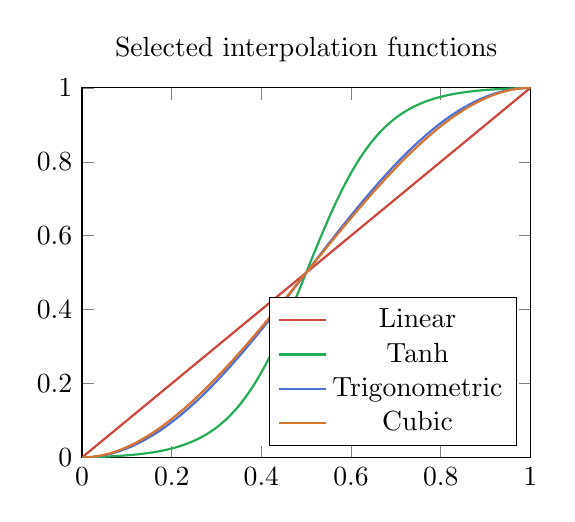
\begin{tikzpicture}
        \begin{axis}[
    align=center,
    title={Selected interpolation functions},
    xmin=0, xmax=1,
    ymin=0, ymax=1,
    domain=0:1,
    xtick={0,0.2,0.4,0.6,0.8,1},
    ytick={0,0.2,0.4,0.6,0.8,1},
    legend pos=south east,
    width=.6\textwidth,
    every axis plot/.append style={thick},
]

    \addplot[mark=none,color=softred,samples=2] { x };
    \addlegendentry{Linear}

    \addplot[mark=none,color=softgreen,samples=300] { .5 * tanh(6*x-3)/tanh(3) + .5 };
    \addlegendentry{Tanh}
    
    \addplot[mark=none,color=softblue,samples=300] { .5 * (1 - cos(pi * deg(x))) };
    \addlegendentry{Trigonometric}
    
    \addplot[mark=none,color=softorange,samples=300] { 3*x^2 - 2*x^3 };
    \addlegendentry{Cubic}

\end{axis}

    \end{tikzpicture}
    \caption{Comparison of the four selected interpolation functions}
\end{figure}

Later experiments explore the effects of rapid changes in airway constriction. To move between these
``constricted'' and ``unconstricted'' states, we have four different interpolation functions:

\begin{itemize}
    \item \textit{Linear}: $f(x) = x$
    \item \textit{Tanh}: $f(x) = \frac{1}{2} \frac{\tanh(6x - 3)}{\tanh(3)} + \frac{1}{2}$
    \item \textit{Trigonometric}: $f(x) = \frac{1}{2} (1 - \cos(\pi x))$
    \item \textit{Cubic}: $f(x) = 3x^2 - 2x^3$
\end{itemize}

\noindent
A visual comparison of these functions is provided in \autoref{fig:interpolate-functions}.

These functions were selected for their relative simplicity and variety of curvature.

\todo{
    Explaining exactly why the curvature is necessary is escaping me right now. It's basically that
    the flow behaves extra weirdly without curvy interpolation, but that's not very scientific.

    There's an alternate angle, which is that curvy interpolation intentionally allows the
    significant changes at high constriction to happen more slowly (e.g. going 10\% to 15\% is much
    slower than 15\% to 20\%). This is ``good'' because flow characteristics change rapidly as you
    change constriction \textit{from} high constrictions, so moving slowly ensures that the flow is
    less erratic.

    On the other hand, maybe this is biasing the results and \textit{actually} the erratic flow is
    more realistic. Would be good to discuss.
}

\todo{
    The other piece of writing in this section is going to be a comparison of the flow
    characteristics when when switching on various interpolation methods.

    We eventually choose \textit{Tanh}, basically because it looks the best (subject to change!).
    See above notes.
}

\breakpars

Finally, it is worth noting that the correction factor of $\tanh(3)$ in the denominator of the
\textit{Tanh} interpolation function is nearly equal to 1, but still necessary. The value of
$\tanh(3)$ is only 0.995, but experiments without that correction factor showed clearly visible
instantaneous changes in flow from that small change. While these changes were most likely harmless,
we still elected to remove them.

\newpage

\todo{
    Here's an outline of the remaining items I'd like to put in this section, in a rough order:
}

\begin{itemize}
    \item Stable flow characteristics of lungs with varying degradation
        \begin{itemize}
            \item Basically just want to point out the ways that the curve starts to become
                lopsided and out of phase from the pleural pressure, with particular emphasis on
                the way that the effect starts rapidly heightening as the constriction
                approaches 10\% (about~--~I haven't tested beyond that, which I should).
        \end{itemize}
    \item Onset and recovery from airflow constriction. Key things are:
        \begin{itemize}
            \item Just showing off the simple graphs, to get a sense of what's going on
            \item Slow recovery reduces strain~--~we can get abnormally high airflow if pleural
                pressure lines up with suddenly-reduced constriction 
            \item Relating to above: I'd like to have a version of the crazy graph~--~the one
                where it's all just ``degrade and recover'', with each startpoint being offset
                by 0.5s from the previous one. It would be really good to align that with some
                kind of chart showing the minimum and maximum flow velocity reached (on top of
                the normal min/max), to show the kind of chance of risk we run~--~and how much
                that reduces as the recovery becomes slower.
            \item Flow characteristics align with those from the current level of constriction
                (i.e. on the way to 10\%, the area around 20\% constriction tends to mimic the
                flow characteristics from 20\% at that point)
            \item The above points are probably three distinct sub-sections.
        \end{itemize}
\end{itemize}


\newpage
\bibliography{ref.bib}{}
\bibliographystyle{plain}

\end{document}
